\section{Control Structures}

\begin{concept}{Branch Instructions}\\
Branch instructions control program flow:

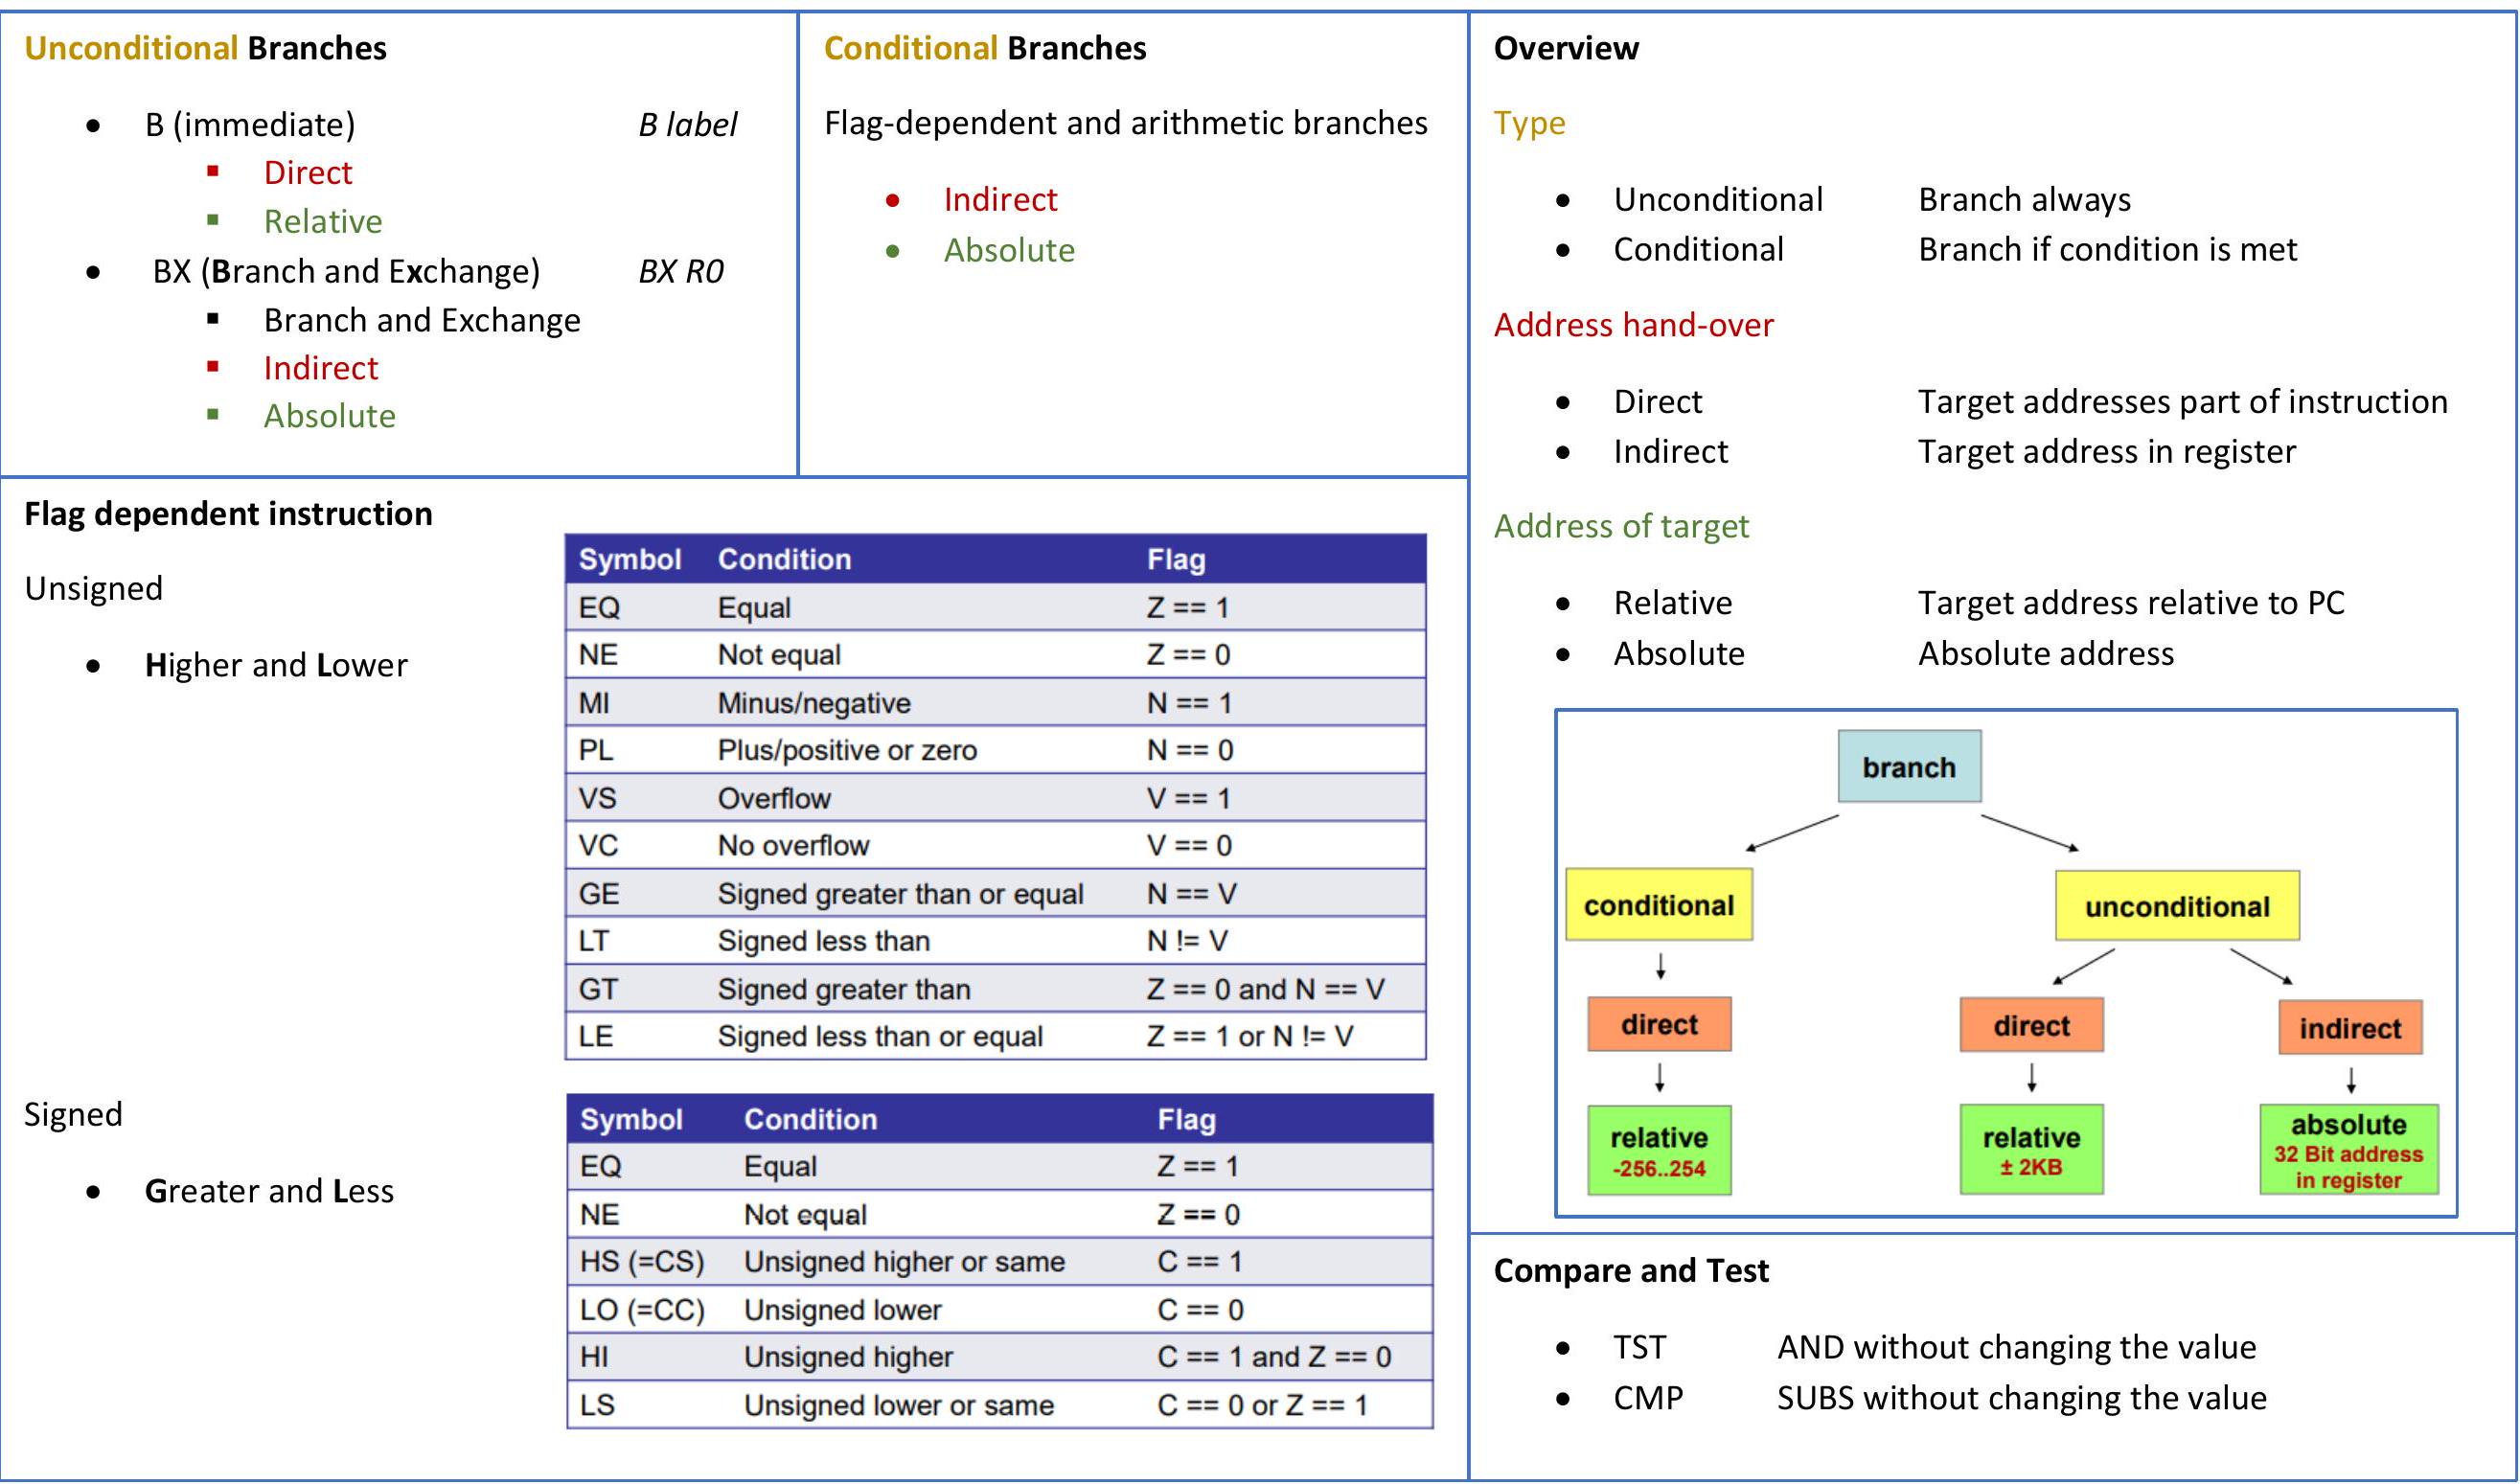
\includegraphics[width=\linewidth]{images/2024_12_29_79e6b22f503fb7b4f718g-05}

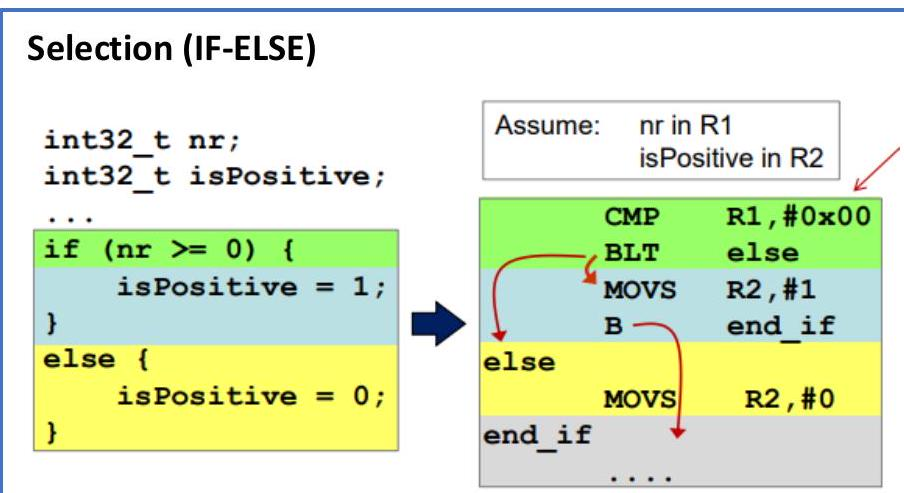
\includegraphics[width=\linewidth]{images/2024_12_29_79e6b22f503fb7b4f718g-07(3)}
\end{concept}

\begin{example2}{Switch Statement Implementation}
C code example:
\begin{lstlisting}[language=C, style=basesmol]
uint32_t result, n;
switch (n) {
    case 0:
        result += 17;
        break;
    case 1:
        result += 13;
        //fall through
    case 3: 
    case 5:
        result += 37;
        break;
    default:
        result = 0;
}
\end{lstlisting}

Assembly implementation with jump table:
\begin{lstlisting}[language=armasm, style=basesmol]
NR_CASES    EQU     6
case_switch CMP     R1, #NR_CASES
            BHS     case_default
            LSLS    R1, #2        ; * 4
            LDR     R7, =jump_table
            LDR     R7, [R7, R1]
            BX      R7

case_0      ADDS    R2, R2, #17
            B       end_sw_case
case_1      ADDS    R2, R2, #13
case_3_5    ADDS    R2, R2, #37
            B       end_sw_case
case_default MOVS   R2, #0
end_sw_case ...

jump_table  DCD     case_0
            DCD     case_1
            DCD     case_default
            DCD     case_3_5
            DCD     case_default
            DCD     case_3_5
\end{lstlisting}
\end{example2}

\begin{concept}{Loop Types}\\
Three main types of loops:

\textbf{Do-While (Post-Test Loop)}:
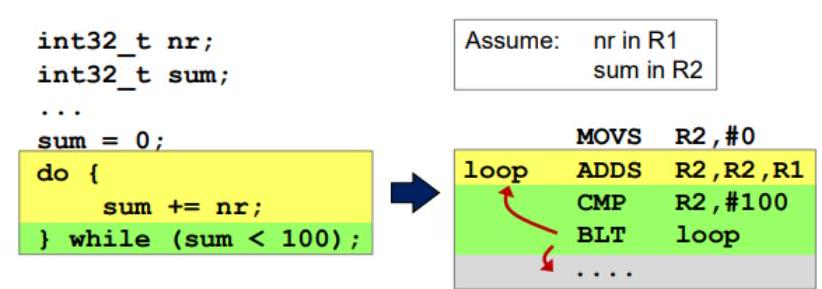
\includegraphics[width=\linewidth]{images/2024_12_29_79e6b22f503fb7b4f718g-07}

\textbf{While (Pre-Test Loop)}:
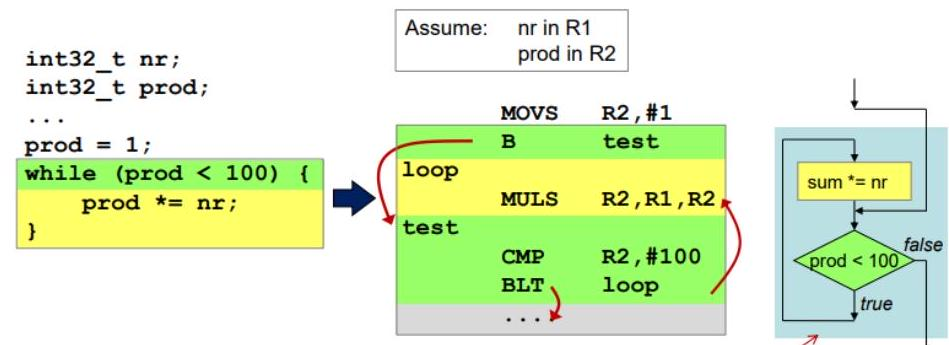
\includegraphics[width=\linewidth]{images/2024_12_29_79e6b22f503fb7b4f718g-07(1)}

\textbf{For Loop (Pre-Test Loop)}:
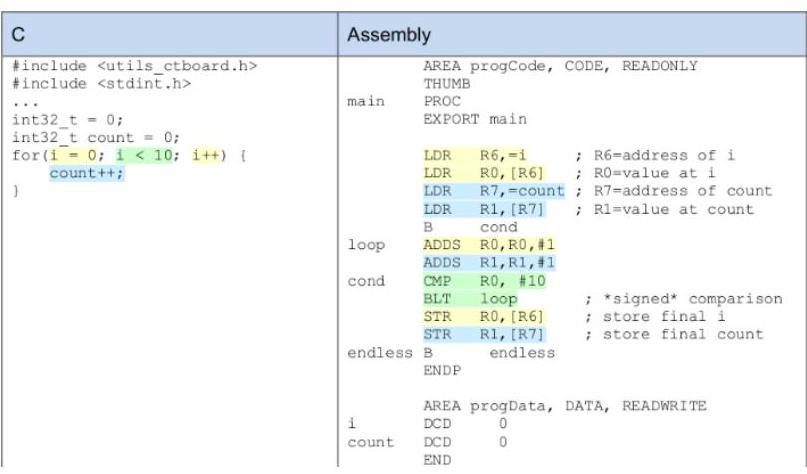
\includegraphics[width=\linewidth]{images/2024_12_29_79e6b22f503fb7b4f718g-07(2)}
\end{concept}

\begin{KR}{Implementing Control Structures}\\
Steps for implementing control structures:
\begin{enumerate}
  \item Choose appropriate control structure:
    \begin{itemize}
      \item If-then-else for simple decisions
      \item Switch for multiple cases with same variable
      \item Loops for repeated operations
    \end{itemize}
  \item For switches:
    \begin{itemize}
      \item Create jump table
      \item Calculate offset based on case value
      \item Handle default case
    \end{itemize}
  \item For loops:
    \begin{itemize}
      \item Initialize counter/condition
      \item Place condition check appropriately
      \item Ensure proper exit condition
      \item Update variables correctly
    \end{itemize}
\end{enumerate}
\end{KR}

\begin{example2}{Basic Control Structures}
Example implementations:
\begin{lstlisting}[language=armasm, style=basesmol]
    ; If-then-else
    CMP     R0, #0      ; Compare value
    BEQ     else_label  ; Branch if equal
    ; then code
    B       endif_label
else_label
    ; else code
endif_label

    ; While loop
    B       while_cond  ; Jump to condition
while_loop
    ; loop body
while_cond
    CMP     R0, #10     ; Check condition
    BLT     while_loop  ; Branch if less than

    ; Do-while loop
do_loop
    ; loop body
    CMP     R0, #10     ; Check condition
    BLT     do_loop     ; Branch if less than
\end{lstlisting}
\end{example2}

\begin{formula}{Branch Instruction Types}\\
Classification of branch instructions:

\textbf{1. Based on Condition:}
\begin{itemize}
  \item \textbf{Unconditional:}
    \begin{itemize}
      \item B - Branch always
      \item BL - Branch with Link
      \item BX - Branch and Exchange
    \end{itemize}
  \item \textbf{Conditional:}
    \begin{itemize}
      \item Flag-dependent (EQ, NE, CS, CC, etc.)
      \item Arithmetic (HI, LS, GE, LT, etc.)
    \end{itemize}
\end{itemize}

\textbf{2. Based on Target Address:}
\begin{itemize}
  \item \textbf{Direct:} Target address in instruction
  \item \textbf{Indirect:} Target address in register
  \item \textbf{Relative:} Offset from current PC
  \item \textbf{Absolute:} Complete target address
\end{itemize}
\end{formula}

\begin{KR}{Selection Implementation}\\
Guidelines for implementing if-then-else structures:

1. Simple if-then:
\begin{lstlisting}[language=armasm, style=base]
    ; if (x > 0) { x++; }
    CMP     R0, #0          ; Compare x with 0
    BLE     endif           ; Skip if x <= 0
    ADDS    R0, #1          ; x++
endif
\end{lstlisting}

2. if-then-else:
\begin{lstlisting}[language=armasm, style=base]
    ; if (x > y) { x = y; } else { y = x; }
    CMP     R0, R1          ; Compare x and y
    BLE     else_part       ; Branch if x <= y
    MOVS    R0, R1          ; Then part: x = y
    B       endif           ; Skip else part
else_part
    MOVS    R1, R0          ; Else part: y = x
endif
\end{lstlisting}

3. Nested if:
\begin{lstlisting}[language=armasm, style=base]
    ; if (x > 0) {
    ;     if (y > 0) {
    ;         x = y;
    ;     }
    ; }
    CMP     R0, #0          ; Check x > 0
    BLE     endif_outer
    CMP     R1, #0          ; Check y > 0
    BLE     endif_inner
    MOVS    R0, R1          ; x = y
endif_inner
endif_outer
\end{lstlisting}
\end{KR}

\begin{KR}{Loop Implementation}\\
Templates for different loop types:

1. While loop:
\begin{lstlisting}[language=armasm, style=base]
    ; while (x < 10) { x++; }
    B       while_cond      ; Jump to condition
while_loop
    ADDS    R0, #1          ; x++
while_cond
    CMP     R0, #10         ; Check x < 10
    BLT     while_loop      ; Continue if true
\end{lstlisting}

2. Do-while loop:
\begin{lstlisting}[language=armasm, style=base]
    ; do { x++; } while (x < 10);
do_loop
    ADDS    R0, #1          ; x++
    CMP     R0, #10         ; Check x < 10
    BLT     do_loop         ; Continue if true
\end{lstlisting}

3. For loop:
\begin{lstlisting}[language=armasm, style=base]
    ; for (i = 0; i < 10; i++)
    MOVS    R0, #0          ; i = 0
    B       for_cond
for_loop
    ; Loop body
    ADDS    R0, #1          ; i++
for_cond
    CMP     R0, #10         ; Check i < 10
    BLT     for_loop        ; Continue if true
\end{lstlisting}
\end{KR}

\begin{KR}{Switch Implementation}\\
Steps for implementing switch statements:

1. Range check and table access:
\begin{lstlisting}[language=armasm, style=base]
    CMP     R0, #MAX_CASES  ; Check range
    BHS     default_case    ; If too high, default
    LSLS    R0, #2          ; Multiply by 4
    LDR     R1, =jump_table ; Load table address
    ADD     R1, R0          ; Add offset
    LDR     R1, [R1]        ; Load target address
    BX      R1              ; Branch to case
\end{lstlisting}

2. Jump table structure:
\begin{lstlisting}[language=armasm, style=base]
jump_table
    DCD     case_0          ; Case 0 handler
    DCD     case_1          ; Case 1 handler
    DCD     default_case    ; Default handler
    ; ... more cases
\end{lstlisting}

3. Case handlers:
\begin{lstlisting}[language=armasm, style=base]
case_0
    ; Handle case 0
    B       switch_end
case_1
    ; Handle case 1
    B       switch_end
default_case
    ; Handle default case
switch_end
\end{lstlisting}
\end{KR}

\begin{example2}{Complex Control Structure}
Implementing nested loops with conditions:
\begin{lstlisting}[language=armasm, style=base]
    ; for (i = 0; i < 5; i++) {
    ;     if (i == 2) continue;
    ;     for (j = 0; j < 3; j++) {
    ;         if (j == 1) break;
    ;         sum += i + j;
    ;     }
    ; }
    
    MOVS    R0, #0          ; i = 0
outer_loop
    CMP     R0, #2          ; Check i == 2
    BEQ     outer_continue  ; Skip if i == 2
    
    MOVS    R1, #0          ; j = 0
inner_loop
    CMP     R1, #1          ; Check j == 1
    BEQ     outer_continue  ; Break to outer loop
    
    ADDS    R2, R0, R1      ; Calculate i + j
    ADDS    R4, R4, R2      ; Add to sum
    
    ADDS    R1, #1          ; j++
    CMP     R1, #3          ; Check j < 3
    BLT     inner_loop      ; Continue inner loop
    
outer_continue
    ADDS    R0, #1          ; i++
    CMP     R0, #5          ; Check i < 5
    BLT     outer_loop      ; Continue outer loop
\end{lstlisting}
\end{example2}

\begin{formula}{Branch Instruction Types}\\
Classification of branch instructions:

\textbf{1. Based on Condition:}
\begin{itemize}
  \item \textbf{Unconditional:}
    \begin{itemize}
      \item B - Branch always
      \item BL - Branch with Link
      \item BX - Branch and Exchange
    \end{itemize}
  \item \textbf{Conditional:}
    \begin{itemize}
      \item Flag-dependent (EQ, NE, CS, CC, etc.)
      \item Arithmetic (HI, LS, GE, LT, etc.)
    \end{itemize}
\end{itemize}

\textbf{2. Based on Target Address:}
\begin{itemize}
  \item \textbf{Direct:} Target address in instruction
  \item \textbf{Indirect:} Target address in register
  \item \textbf{Relative:} Offset from current PC
  \item \textbf{Absolute:} Complete target address
\end{itemize}
\end{formula}

\begin{KR}{Selection Implementation}\\
Guidelines for implementing if-then-else structures:

1. Simple if-then:
\begin{lstlisting}[language=armasm, style=base]
    ; if (x > 0) { x++; }
    CMP     R0, #0          ; Compare x with 0
    BLE     endif           ; Skip if x <= 0
    ADDS    R0, #1          ; x++
endif
\end{lstlisting}

2. if-then-else:
\begin{lstlisting}[language=armasm, style=base]
    ; if (x > y) { x = y; } else { y = x; }
    CMP     R0, R1          ; Compare x and y
    BLE     else_part       ; Branch if x <= y
    MOVS    R0, R1          ; Then part: x = y
    B       endif           ; Skip else part
else_part
    MOVS    R1, R0          ; Else part: y = x
endif
\end{lstlisting}

3. Nested if:
\begin{lstlisting}[language=armasm, style=base]
    ; if (x > 0) {
    ;     if (y > 0) {
    ;         x = y;
    ;     }
    ; }
    CMP     R0, #0          ; Check x > 0
    BLE     endif_outer
    CMP     R1, #0          ; Check y > 0
    BLE     endif_inner
    MOVS    R0, R1          ; x = y
endif_inner
endif_outer
\end{lstlisting}
\end{KR}

\begin{KR}{Loop Implementation}\\
Templates for different loop types:

1. While loop:
\begin{lstlisting}[language=armasm, style=base]
    ; while (x < 10) { x++; }
    B       while_cond      ; Jump to condition
while_loop
    ADDS    R0, #1          ; x++
while_cond
    CMP     R0, #10         ; Check x < 10
    BLT     while_loop      ; Continue if true
\end{lstlisting}

2. Do-while loop:
\begin{lstlisting}[language=armasm, style=base]
    ; do { x++; } while (x < 10);
do_loop
    ADDS    R0, #1          ; x++
    CMP     R0, #10         ; Check x < 10
    BLT     do_loop         ; Continue if true
\end{lstlisting}

3. For loop:
\begin{lstlisting}[language=armasm, style=base]
    ; for (i = 0; i < 10; i++)
    MOVS    R0, #0          ; i = 0
    B       for_cond
for_loop
    ; Loop body
    ADDS    R0, #1          ; i++
for_cond
    CMP     R0, #10         ; Check i < 10
    BLT     for_loop        ; Continue if true
\end{lstlisting}
\end{KR}

\begin{KR}{Switch Implementation}\\
Steps for implementing switch statements:

1. Range check and table access:
\begin{lstlisting}[language=armasm, style=base]
    CMP     R0, #MAX_CASES  ; Check range
    BHS     default_case    ; If too high, default
    LSLS    R0, #2          ; Multiply by 4
    LDR     R1, =jump_table ; Load table address
    ADD     R1, R0          ; Add offset
    LDR     R1, [R1]        ; Load target address
    BX      R1              ; Branch to case
\end{lstlisting}

2. Jump table structure:
\begin{lstlisting}[language=armasm, style=base]
jump_table
    DCD     case_0          ; Case 0 handler
    DCD     case_1          ; Case 1 handler
    DCD     default_case    ; Default handler
    ; ... more cases
\end{lstlisting}

3. Case handlers:
\begin{lstlisting}[language=armasm, style=base]
case_0
    ; Handle case 0
    B       switch_end
case_1
    ; Handle case 1
    B       switch_end
default_case
    ; Handle default case
switch_end
\end{lstlisting}
\end{KR}

\begin{example2}{Complex Control Structure}
Implementing nested loops with conditions:
\begin{lstlisting}[language=armasm, style=base]
    ; for (i = 0; i < 5; i++) {
    ;     if (i == 2) continue;
    ;     for (j = 0; j < 3; j++) {
    ;         if (j == 1) break;
    ;         sum += i + j;
    ;     }
    ; }
    
    MOVS    R0, #0          ; i = 0
outer_loop
    CMP     R0, #2          ; Check i == 2
    BEQ     outer_continue  ; Skip if i == 2
    
    MOVS    R1, #0          ; j = 0
inner_loop
    CMP     R1, #1          ; Check j == 1
    BEQ     outer_continue  ; Break to outer loop
    
    ADDS    R2, R0, R1      ; Calculate i + j
    ADDS    R4, R4, R2      ; Add to sum
    
    ADDS    R1, #1          ; j++
    CMP     R1, #3          ; Check j < 3
    BLT     inner_loop      ; Continue inner loop
    
outer_continue
    ADDS    R0, #1          ; i++
    CMP     R0, #5          ; Check i < 5
    BLT     outer_loop      ; Continue outer loop
\end{lstlisting}
\end{example2}